% !TEX root = mythesis.tex

%==============================================================================
\chapter{The LHC and the ATLAS experiment}
\label{chap:lhcandatlas}

In this chapter, the overall experimental setup is discussed. The Large Hadron Collider (LHC) which is the world's largest and the most powerful particle accelerator is discussed in section \ref{sec:largehadroncollider}. Furthermore, the main setup of the ATLAS detector, which is one of the two general-purpose detectors at the LHC is discussed in section \ref{sec:ATLAS}.

\section{The LHC}
\label{sec:largehadroncollider}

\begin{figure}[!h]
\centering
\includegraphics[width=0.7\textwidth]{ubonn-thesis/Chapters/Chapters_03/Figure/LHC.jpg}
\caption{The CERN Accelerator Complex and its pre-accelerator chain as well as the location of the four main experiments\cite{Haffner:1621894}. The LHC is the large blue ring, which is fed from its predecessor the Super Proton Synchrotron (SPS), shown in light blue, in turn fed from its own predecessor the Proton Synchrotron (PS), in magenta. }
%
\label{fig:LHC}
\end{figure}

The \textbf{L}arge \textbf{H}adron \textbf{C}ollider (LHC), located at the European Organization for Nuclear Research (CERN), is largest and most energetic particle collider ever constructed. It is currently operating at a record center-of-mass energy ($\sqrt{s}$) of 13 tera-electron-Volts (TeV) for proton-proton (pp) collisions. It allows scientists to reproduce the conditions that existed within a billionth of a second after the Big Bang by colliding beams of high-energy protons or ions at colossal speeds, close to the speed of light. Figure \ref{fig:LHC} gives an overview of the CERN accelerator complex. The LHC consists of a 27-kilometer ring of superconducting magnets with a number of accelerating structures to boost the energy of the particles along the way. Inside the accelerator, the particles are accelerated in opposite directions in two rings before they are made to collide. Before the particles are injected inside the beam pipes, they are injected into a linear accelerator (Linac 2) and are accelerated to an energy of 50 MeV. During this first acceleration, the protons are split into bunches. Then, they are injected into the Proton Synchroton Booster (PSB). From there, the protons are led to the Proton Synchroton (PS) with an energy of 1.4 GeV. Their energy is futher increased to 25 GeV, and they are then injected to the Super Proton Synchroton (SPS). Finally, the proton bunches pass to the LHC ring with an energy of 450 GeV, where they are accelerated to the desired energy. During Run I, the LHC operated at a center-of-mass energy of $\sqrt{s}$=7 TeV (2011) and at $\sqrt{s}$=8 TeV (2012). For Run II (2015-2018), the energy was increased to 13 TeV. The beams inside the LHC are made to collide at four locations around the accelerator ring, corresponding to the positions of four particle detectors ATLAS, CMS, ALICE and LHCb (see figure \ref{fig:LHC} ). The ATLAS and CMS detectors are cylindrically symmetrical multi-purpose detectors, which investigate a wide range of physics, from the search for the Higgs boson to extra dimensions and particles that could make up dark matter.

\section{The ATLAS detector}
\label{sec:ATLAS}


\begin{figure}[!h]
\centering
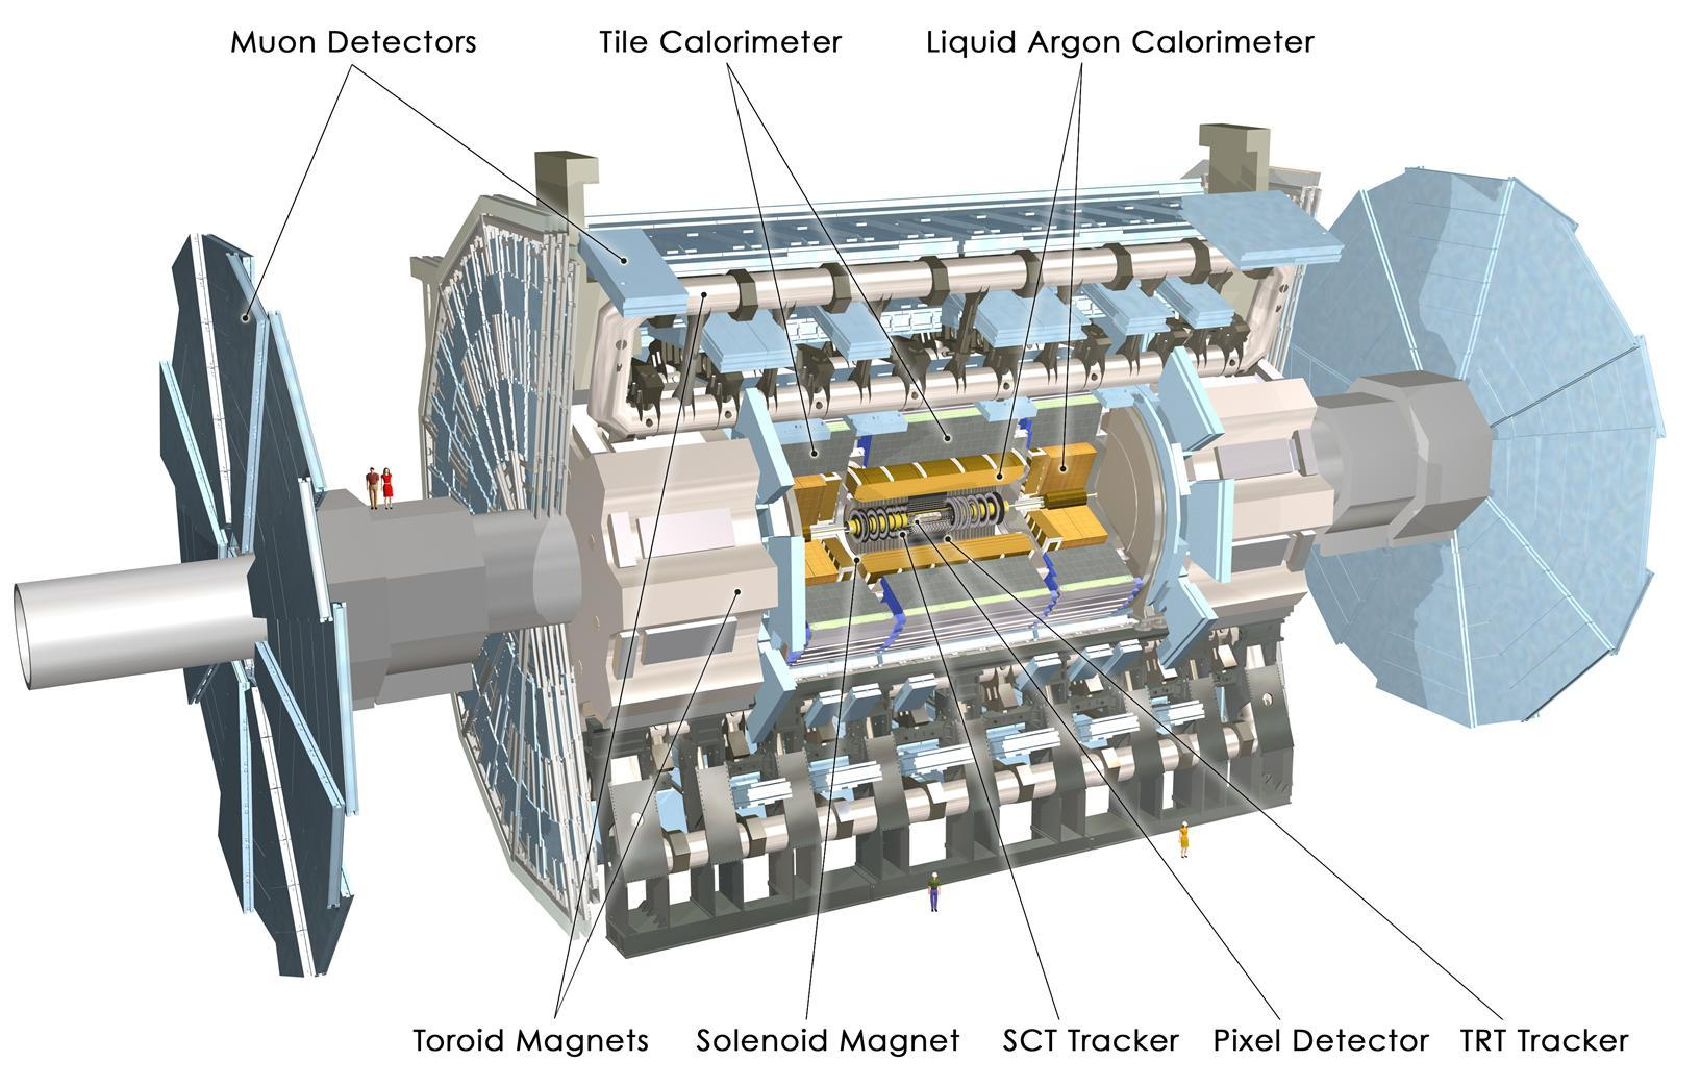
\includegraphics[width=0.6\textwidth]{ubonn-thesis/Chapters/Chapters_03/Figure/ATLAS_detector.pdf}
\caption{Overview over the entire ATLAS detector and its components \cite{PequenaoA}}
\label{fig:atlasdetector}
\end{figure}

The ATLAS detector (\textbf{A} \textbf{T}oroidal \textbf{L}HC \textbf{A}pparatu\textbf{S}) is one of the two largest particle detectors located at the LHC with a length of 44 meters, a diameter of 25 meters and 7000 tonnes of weight as shown in figure \ref{fig:atlasdetector}. It is the detector that is used to take the data for the analysis presented in this thesis and will also be assumed for the detector simulation of the Monte Carlo samples. The different detecting subsystems are arranged in layers around the collision point to record the paths, momentum, and energy of the particles, allowing them to be individually identified. It consists of three main detector components: the inner detector, the calorimeter system, and the muon spectrometer as shown in figure \ref{fig:atlasdetector} . Additionally, the inner detector contains several toroidal and solenoidal magnets whose purpose is to bend charged particles (see figure \ref{fig:atlasdetector} ). Charged particles such as leptons, charged mesons or charged hadrons can be detected through a combination of inner detector tracking and calorimeter deposits. Photons, neutral mesons or neural hadrons can be identified due to their deposits in calorimeter paired with missing curved tracking information from the inner detector. Neutrinos do not interact with the detector components and are inferred by summing all transverse momentum to determine a "missing" energy. A schematic diagram of different particles interacting with the detector components is shown in figure \ref{fig:particleinteraction}. 

\begin{figure}[!h]
\centering
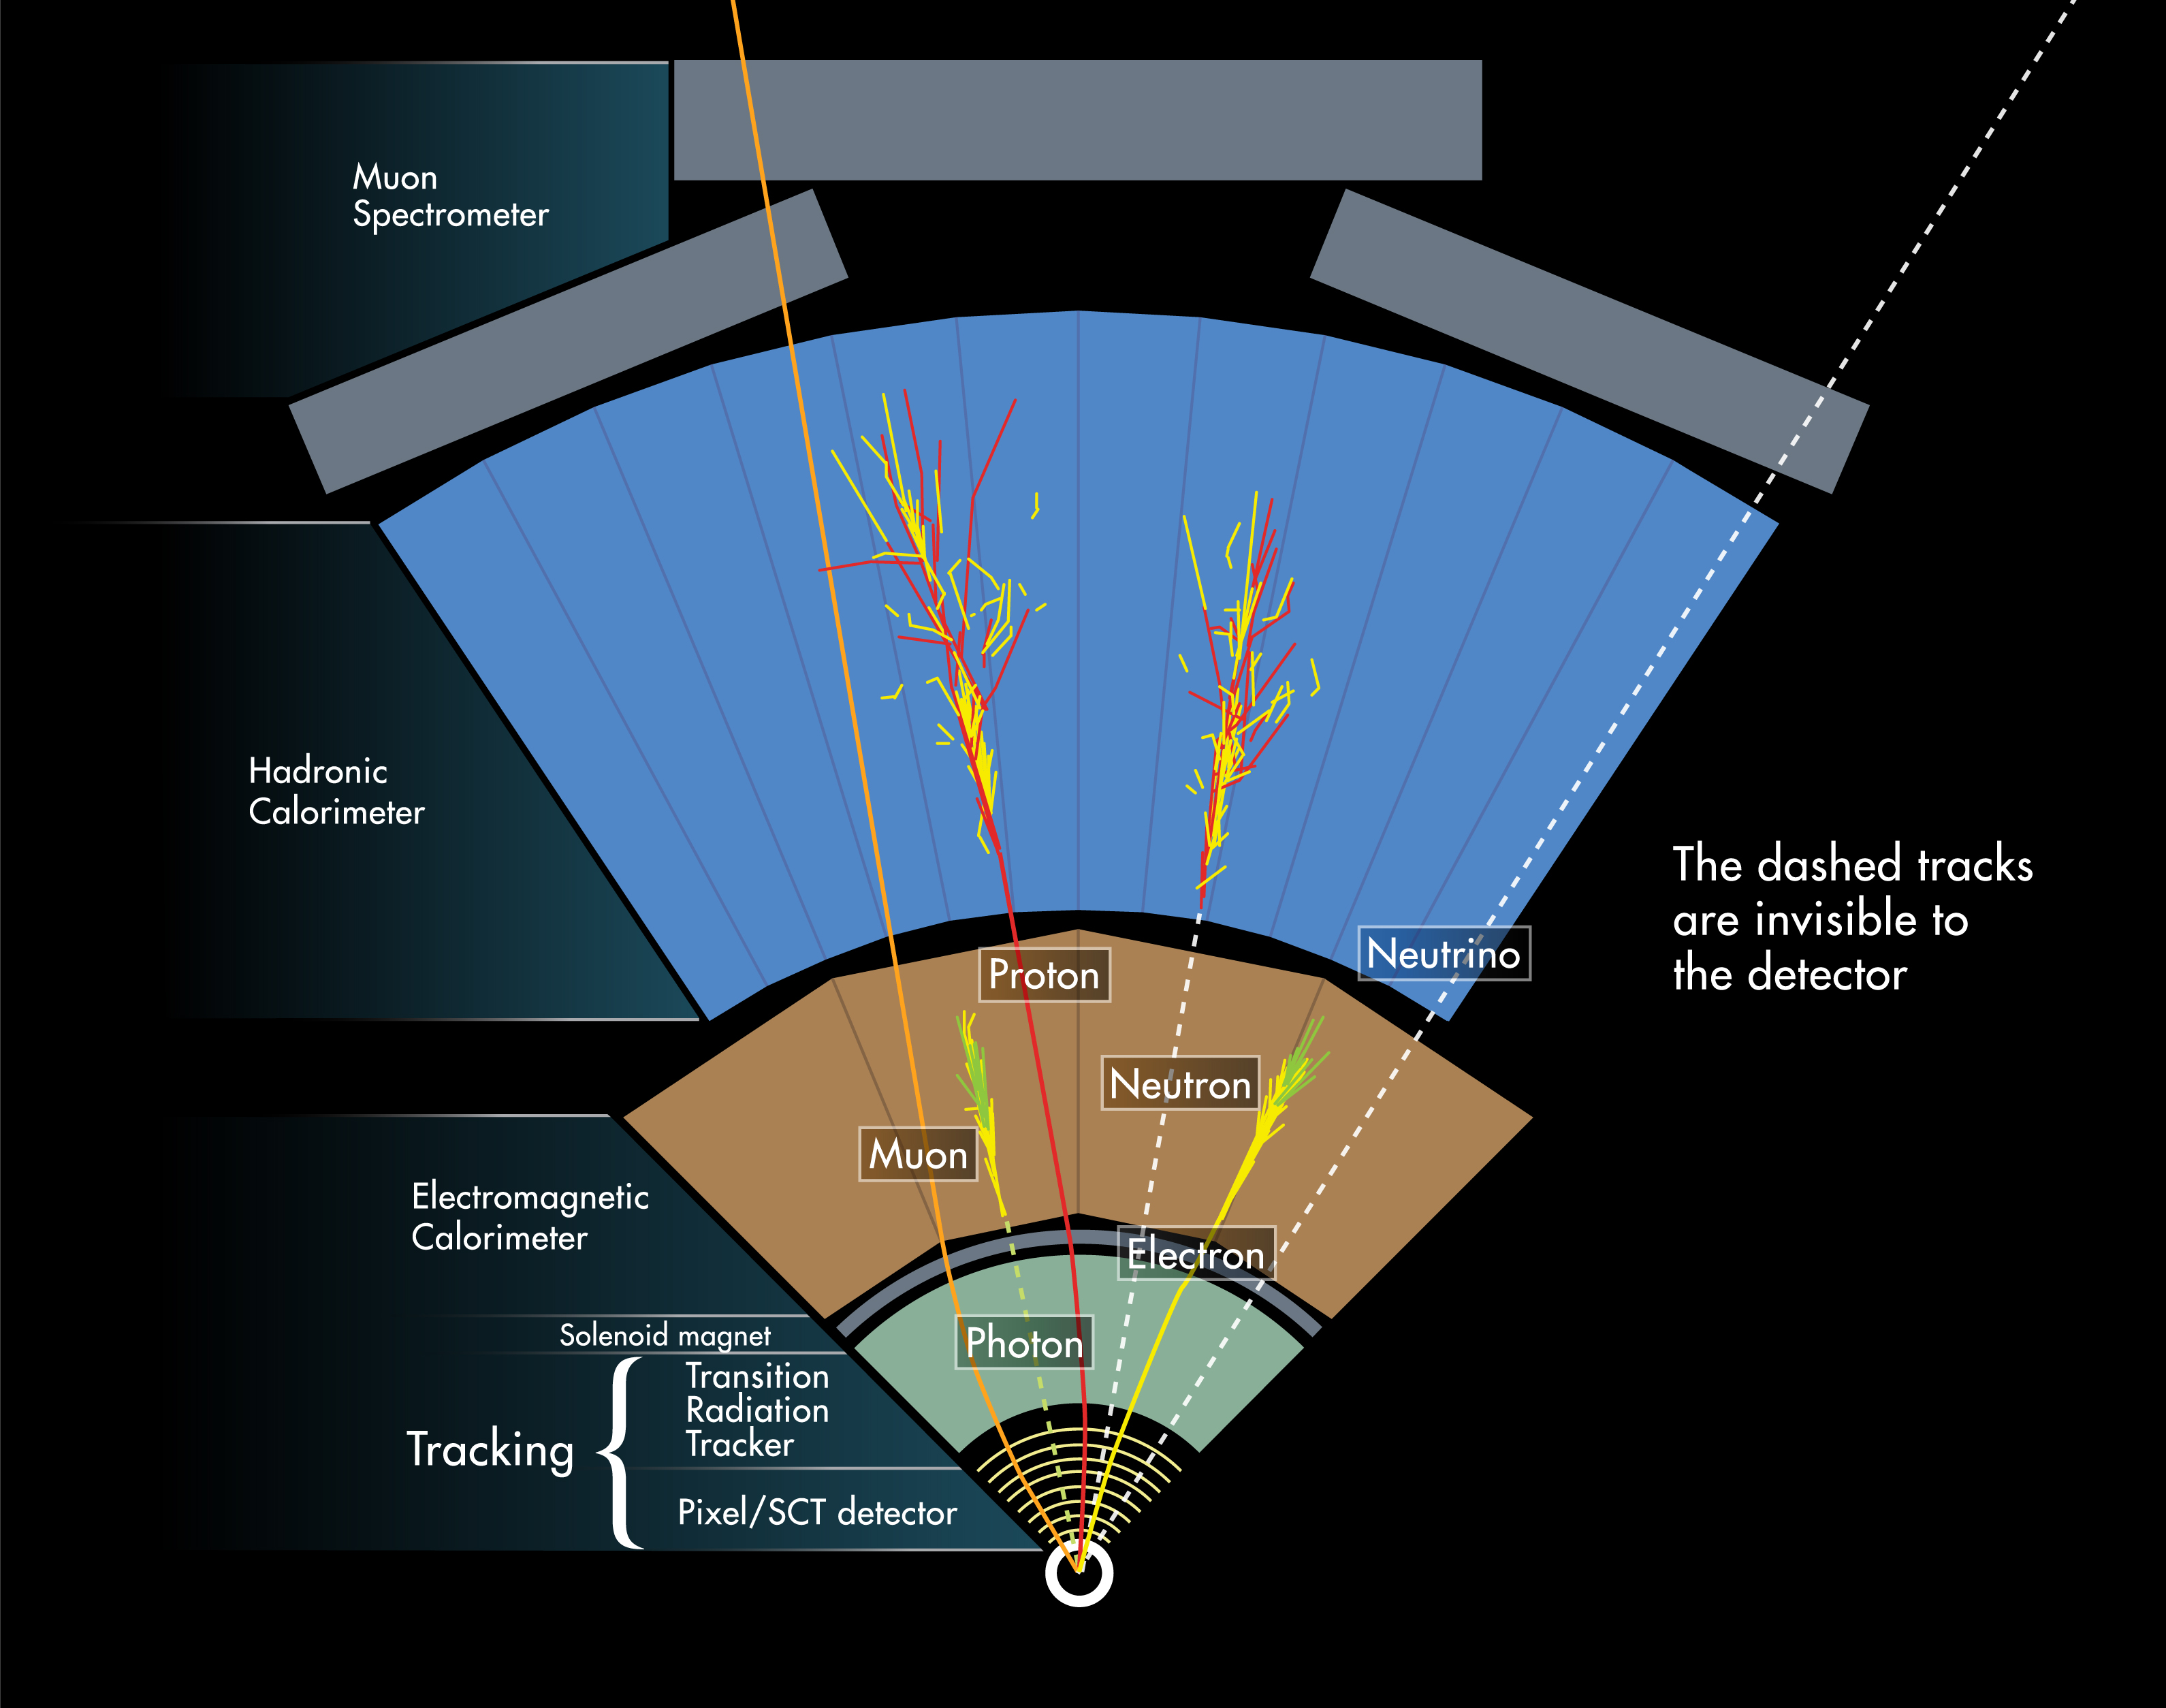
\includegraphics[width=0.6\textwidth]{ubonn-thesis/Chapters/Chapters_03/Figure/Particle_interaction.jpg}
\caption{ Depiction of the detectable particles upon a cross section of the ATLAS detector. \cite{PequenaoB}}
\label{fig:particleinteraction}
\end{figure}


\subsection{The ATLAS coordinate system}
\label{atlascoordinate}
ATLAS makes use of a right-handed coordinate system. The coordinate system has its origin at the nominal interaction point, with the z-axis pointed along the beamline. The x-y plane is transverse to the beam direction, with the positive x-axis pointing towards the center of the LHC ring and the positive y-axis defined as pointing upwards. Due to the symmetry, cylindrical coordinates are used, where $\phi$ is the angle along the plane transverse to the beam with respect to the x-axis and $\theta$ is the polar angle. Instead of the polar angle, pseudorapidity is used, which is defined as

\begin{equation}
    \label{pseudorapidity}
    \eta = - ln ( tan \frac{\theta}{2})
\end{equation}

The distance between two particles or objects in the $\eta$-$\phi$ plane is defined as
\begin{equation}
    \label{deltaR}
    \Delta R = \sqrt{(\Delta \eta)^{2} + (\Delta \phi)^{2}}
\end{equation}


\subsection{Inner detector}

\begin{figure}[!h]
\centering
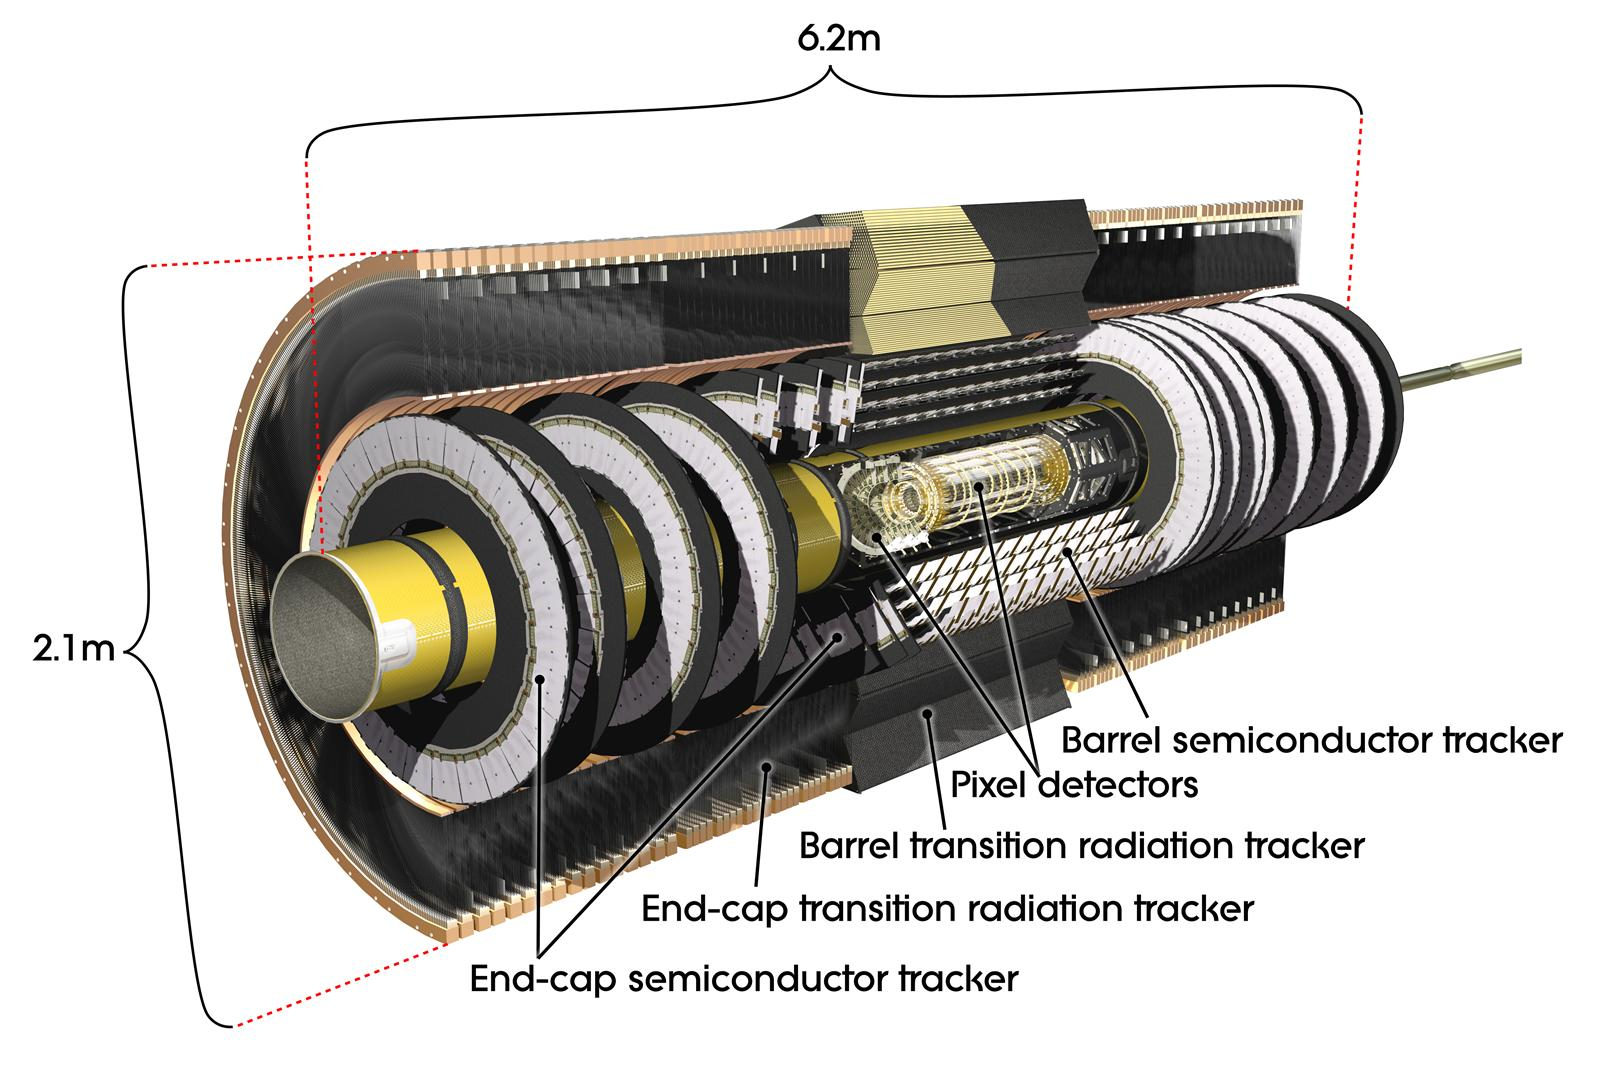
\includegraphics[width=0.6\textwidth]{ubonn-thesis/Chapters/Chapters_03/Figure/inner_detector.jpg}
\caption{ Cut-away view of the ATLAS inner detector \cite{Pequenao:1095926}}
\label{fig:atlasinnerdetector}
\end{figure}

The inner detector is the compact and highly sensitive part of the ATLAS detector that is used to measure the direction, momentum, and charge of electrically-charged particles produced in each proton-proton collision. It consists of three different systems of sensors, all immersed in a magnetic field of 2 T produced by a solenoid located between the tracking system and the calorimeter, parallel to the beam axis. The magnetic field bends the tracks of charged particles allowing a measurement of their momentum. The main components of the inner detector are Pixel Detector, Semiconductor Tracker (SCT), and Transition Radiation Tracker (TRT) as shown in figure \ref{fig:atlasinnerdetector}. 

The pixel detector is the inner part of the detector which is divided into barrel part and an end-cap region covering the range of $|\eta|$<2.5. The barrel region starts 5 cm away from the interaction point making it the detector subsystem closest to the beam pipe. There are four barrel layers with 1736 sensor modules. In the end-cap region, each site constitutes three detector discs oriented perpendicular to the beam pipe with 288 modules. The individual module consists of pixels with size of 50\times400 $\mu m^{2}$ in the external layers and 50\times250 $\mu m^{2}$ in the innermost layers. Thus, the pixel detector plays an important role in the reconstruction of primary and secondary vertices, the latter being useful information for b-tagging.

SCT consists of stereo silicon strips forming four concentic cylinders and nine end-cap discs on each side. It consists of a total of almost 16000 strip sensors, each 6.4 cm long and having an 80 $\mu m$ pitch. It helps in simultaneous measurement of R and $\phi$. TRT is the outer-most part of the inner detector that helps in precision measurement and provides an additional information on the particle type (pions or electrons) that flew through the detector. It consists of thin straw tubes with a diameter of 4 mm, which contain a 0.03 mm thin gold-plated tungsten wire in the centre. They are filled with a gas mixture of Xe, CO$_{2}$, and O$_{2}$.

\subsection{Calorimetry}
\label{sec:calorimetry}

\begin{figure}[!h]
\centering
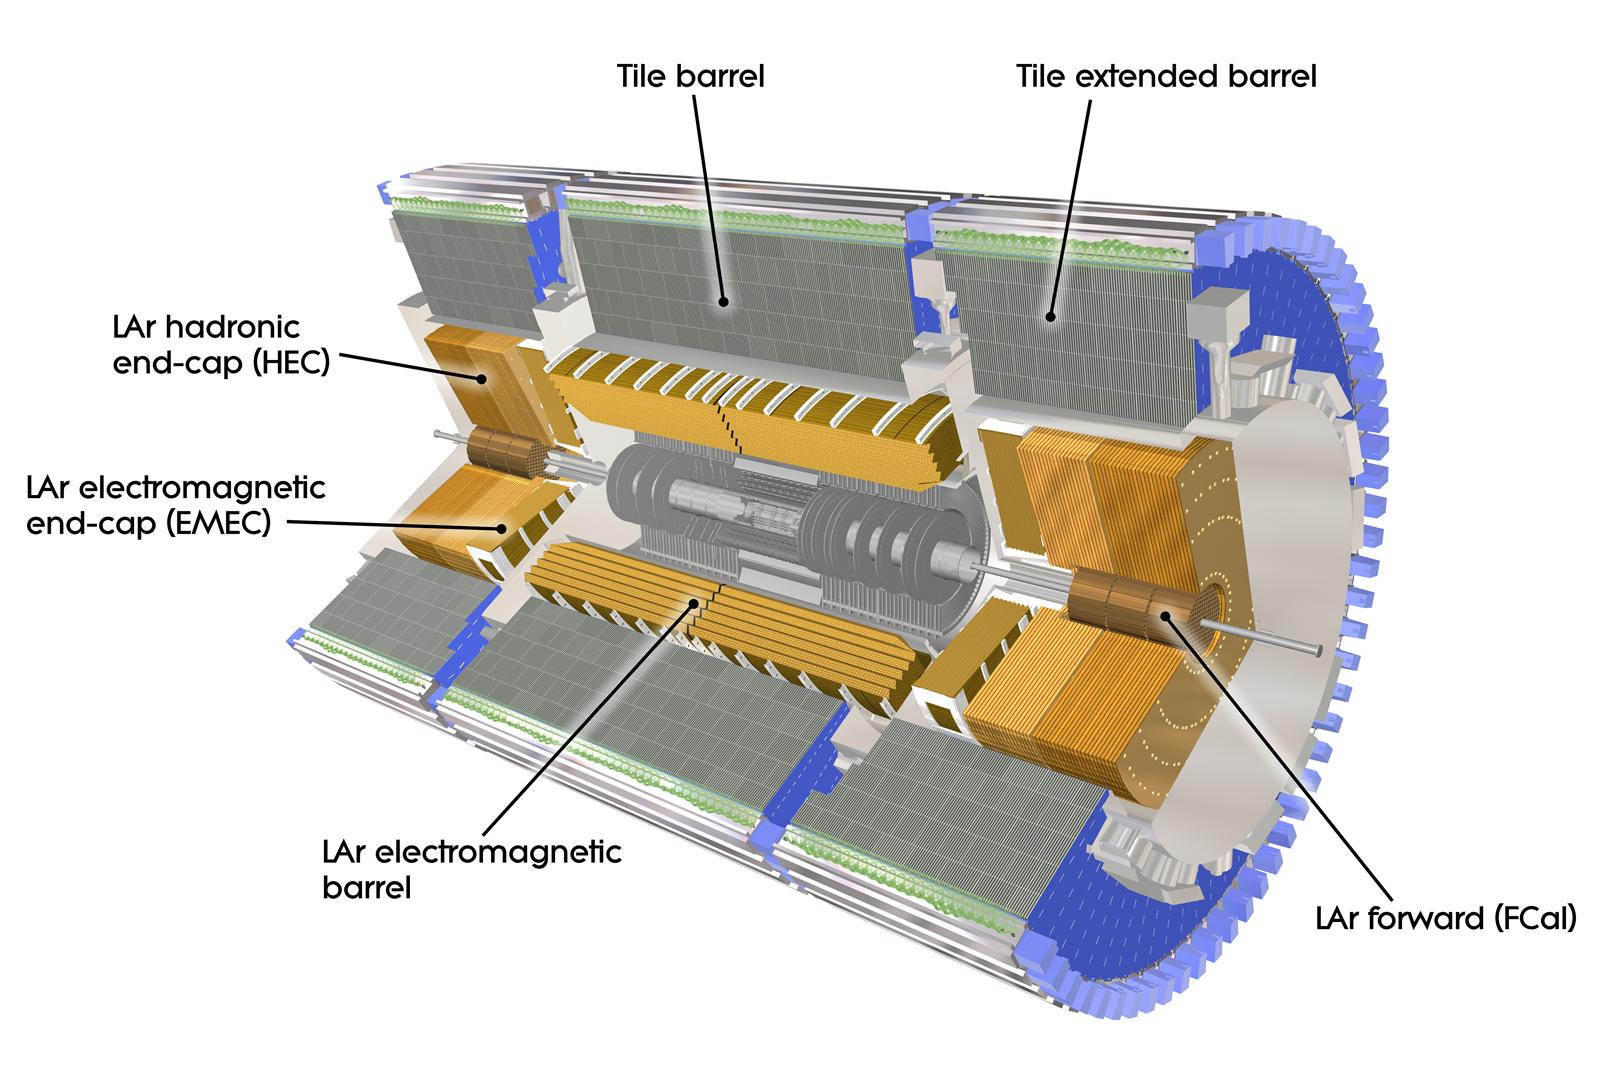
\includegraphics[width=0.6\textwidth]{ubonn-thesis/Chapters/Chapters_03/Figure/calorimeter.jpg}
\caption{Cut-away view of the ATLAS calorimeter \cite{Pequenao:1095927}.}
\label{fig:calorimeter}
\end{figure}


The calorimeter system of the ATLAS detector is divided into 2 subsystems, the inner electromagnetic calorimeter (EMcal) and the outer hadronic calorimeter (Hcal). Both the calorimeters are composed of multiple layers, alternating between an absorber material, which induces particle reactions leading to so called showers and an easy ionizable active material to detect the particles emerging from the absorber material. An overview of the ATLAS calorimeter is shown in figure \ref{fig:calorimeter} . 

EMcal measures the deposited energy of electrons and photons. It is divided into a barrel part and two end-caps. Lead is used as absorber material while liquid argon (LAr) is used as active medium. A combined tile calorimeter and two sample calorimeters in the end-cap regions are used as Hcal. Hcal measures the deposited energy of hadrons. Here, copper is used as active material and LAr as active material. The energy resolution of the calorimeter system can be parametrised as

\begin{equation}
    \label{calorimeter}
     \frac{\sigma(E)}{E} = \frac{a}{\sqrt{E(GeV)}}\oplus b
\end{equation}

For the electromagnetic calorimeter, the corresponding parameters are the stochastic term a $\approx$ 10\% and the constant b $\approx$ 0.7\%, reflecting local non-uniformities in the calorimeter response. For the hadronic calorimeter, the parameters are a $\approx$ 50\% and b $\approx$ 3\% in the barrel and end-cap parts.

\subsection{Muon system}
\label{sec:muonsystem}
Muons are the only SM particles besides neutrinos that escape the inner detector and calorimeters. Muon spectrometer is the outermost layer of the ATLAS detector. It detects muons and measures the properties of their tracks bent in the torodial magnetic field, using high-precision tracking chambers. It is made up of 4,000 individual muon chambers.  It measures the paths of the muons that pass through over a total area the size of a footbal field, to an accuracy of less than one-hundredth of a millimeter. The muon spectrometer is also responsible for the enormous size of the ATLAS detector.





\subsection{Trigger system}
\label{sec:triggersystem}

The ATLAS trigger system selects data in a way that the event at hand contains physics process of interest for the analysis. It consists of the hardware-based level-1 trigger (L1) and the software-based high-level trigger (HLT). Starting with a rate of proton-proton collision events of approximately 40 MHz is reduced to nearly 1 kHz after passing the event filter. The L1 uses a small amount of information from the calorimeters and muon spectrometer to looks for objects and subsequently, regions of interest are built. The HLT is able to access full event data and analyses the regions of interest defined by the L1. After deciding whether to keep the event or not, the events are recorded for physics analysis after passing the event filter.  

\section{Physics objects reconstruction in ATLAS}

In this section, the physics objects that are presented in this thesis is discussed. Electrons, muons, jets, bjets and missing transverse momentum are considered as physics objects. Their definitions are as follow

\subsection{Electrons}
\label{subsec:electron}

Electron candidates are identified using a likelihood-based multivariate method which takes information about the energy deposit in the electromagnetic calorimeter and inner detector tracks. The energy deposit clusters are required to have transverse energy $E_{T}>$ 15 GeV and be found in the pseudorapidity range $|\eta|<$ 2.7 region, excluding the transition region between the barrel and end-cap EMcal found between 1.37 $<|\eta|<$ 1.52. The transverse impact parameter has to fulfill $|d_{0}/\sigma(d_{0})|<$ 5 and $|z_{0}sin(\theta)|<$ 0.5 mm. Here $d_{0}$ and $z_{0}$ refer to the transverse and longitudinal distance of closest approach between the track and the primary vertex. Three quality requirements are available, in order of increasing background rejection power: LooseLH, MediumLH and TightLH. For this analysis all electron candidates are required to pass the TightLH working point. Beyond the quality cut, electrons are required to be isolated using working point discussed in section \ref{subsec:LWP}

\subsection{Muons}
\label{subsec:muons}
Muons are identified by the reconstruction of tracks in the inner detector and the muon spectrometer. To increase background rejection, some additional requirements are placed placed on track-parameter quality in the order of increasing background rejection power: Loose, Medium and Tight. They also have to fulfil $|d_{0}/\sigma(d_{0})|<$ 3 and $|z_{0}sin(\theta)|<$ 0.5 mm. Muon candidates for this analysis pass the Medium identification working point.


\subsection{Jets}
Jets which represent cascades of matter generated in the process of quark hadronization are reconstructed from topological calorimeter clusters using the anti-k$_{t}$ algorithm with a radius parameter of 0.4. They are required to have $P_{T}>$ 35 GeV and $|\eta|<$ 4.5. To suppress jets from pile-up, the Jet Vertex Tagger (JVT) is used.

\subsection{b-jets}
Identifying b-jets, which are jets from hadrons containing bottom quarks, is crucial for analyses with top quarks, since the top quark decays in almost 100\% of all cases into a W boson and a bottom quark. b-jets are identified with the DL1r algorithm. Specially DL1r$\_$PC variant is used; corresping to the current recommendation. The chosen working point is 70\% due to the optimal signal to background ratio.

\subsection{Missing transverse energy}
Missing transverse momentum $E_{T}^{miss}$ is defined as the magnitude of the transverse momentum vector which quantifies the transverse momentum imbalance of all detectable momenta. Since neutrinos will pass the ATLAS detector without interacting with any of its sub-detectors, events containing neutrinos will contain $E_{T}^{miss}$ due to energy-momentum conservation. The $E_{T}^{miss}$ is calculated as the magnitude of the negative sum of the transverse momenta of all identified jets, electrons and muons in the event, as well as soft term built from tracks that are associated to the hard-scatter vertex but are not associated to any of the reconstructed objects. 
